%===============================================================================
%===============================================================================
%
\clearpage
%
\subsection{Example-0401}
%
%===============================================================================
%
\subsubsection{Mathematical model}
%
We solve the Monodomain Equation
%
\begin{align}
    \sigma \Delta V_m(t) = A_m\Big(C_m \dfrac{\partial V_m}{\partial t} + I_{ionic}(V_m)\Big) & &&\Omega = [0, 1] \times [0, 1], \quad t \in [0, 3.0]
\end{align}
%
where $V_m(t)$ is given by the Hodgkin-Huxley system of ODEs

with boundary conditions
%
\begin{align}
    V_m = 0 & &&x = y = 0, \\
    V_m = 0 & &&x = y = 1.
\end{align}
and initial values 
%
\begin{equation*}
  \begin{array}{lll}
    V_m(t=0) = -75
  \end{array}
\end{equation*}
%
Additionally a stimulation current $I_{stim}$ is applied for $t_{stim} = [0, 0.1]$ at the center node of the domain (i.e. at $(x,y) = (\frac12, \frac12,)$).
%

Material parameters:
\begin{equation*}
  \begin{array}{lll}
    \sigma = 3.828\\[4mm]
    A_m = 500\\[4mm]
    C_m = 0.58 \quad \text{for the slow-twitch case,} \quad C_m = 1.0 \quad \text{for the fast-twitch case}\\[4mm]
    I_{Stim} = 1200 \quad \text{for the slow-twitch case,} \quad I_{Stim} = 2000.0 \quad \text{for the fast-twitch case}\\[4mm]    
  \end{array}
\end{equation*}
%
%===============================================================================
%
\subsubsection{Computational model}
%
\begin{itemize}
    \item{This example uses generated meshes}
    \item{Commandline arguments are:}
        \subitem{number elements X} 		
        \subitem{number elements Y}		
        \subitem{interpolation order (1: linear; 2: quadratic)}
        \subitem{solver type (0: direct; 1: iterative)}	
        \subitem{PDE step size}
        \subitem{stop time}
        \subitem{output frequency} 		
        \subitem{CellML Model URL}
        \subitem{slow-twitch}	
        \subitem{ODE time-step}
    \item{Commands for tests are:}
     \subitem{\verb|./folder/src/example 24 24 1 0 0.005 3.0 1 hodgkin_huxley_1952.cellml F 0.0001|}
     \subitem{\verb|./folder/src/example 24 24 1 0 0.005 3.0 1 hodgkin_huxley_1952.cellml F 0.005|}
     \subitem{\verb|./folder/src/example 10 10 1 0 0.005 3.0 1 hodgkin_huxley_1952.cellml F 0.0001|}
     \subitem{\verb|mpirun -n 2 ./folder/src/example 24 24 1 0 0.005 3.0 1 hodgkin_huxley_1952.cellml F 0.0001|}
     \subitem{\verb|mpirun -n 8 ./folder/src/example 24 24 1 0 0.005 3.0 1 hodgkin_huxley_1952.cellml F 0.0001|}
     \subitem{\verb|./folder/src/example 2 2 1 0 0.005 3.0 1 hodgkin_huxley_1952.cellml F 0.0001|}
     \subitem{\verb|mpirun -n 2 ./folder/src/example 2 2 1 0 0.005 3.0 1 hodgkin_huxley_1952.cellml F 0.0001|}
    \item{This is a dynamic problem.}
\end{itemize}
%
%===============================================================================
%
\subsubsection{Results}
%
%\begin{figure}[h!]
%    \centering 
%    \includegraphics[width=0.9\columnwidth]{examples/example-0001/doc/figures/analytical_solution.eps} 
%    \caption{Results, analytical solution.}
%    \label{example-0001-analytical-solution-fig}
%\end{figure}
%
%\begin{figure}[h!]
%    \centering 
%    \includegraphics[width=0.9\columnwidth]{examples/example-0001/doc/figures/abaqus_reference.eps} 
%    \caption{Results, Abaqus reference.}
%    \label{example-0001-abaqus-reference-fig}
%\end{figure}
%
\verbatiminput{examples/example-0401/results/results.summary}
\verbatiminput{examples/example-0401/results/failed.tests}
%
\begin{figure}[ht]
  \centering 
  
%  
% the following works in Adobe Acrobat Reader with \usepackage{movie15}
%\includemovie[     
%  poster,
%  text={\small(Loading)}
%]{6cm}{6cm}{examples/example-0401/doc/figures/current_run_l1x1_n24x24_i1_s0_p1_.mp4}
%
%
% the following works in Adobe Acrobat Reader with \usepackage{media9}
  \includemedia[
    width=0.9\linewidth,
    height=0.9\linewidth,
    activate=pageopen,
    addresource=examples/example-0401/doc/figures/current_run_l1x1_n24x24_i1_s0_p1_.mp4,
    flashvars={source=examples/example-0401/doc/figures/current_run_l1x1_n24x24_i1_s0_p1_.mp4}
  ]{}{VPlayer.swf}
  \caption{Results movie, $24 \times 24$ elements (only works in certain pdf viewers, e.g. Adobe Acrobat Reader)}
  \label{example-0401-current-run0-fig}
\end{figure}

\begin{figure}[ht]
  \centering 
  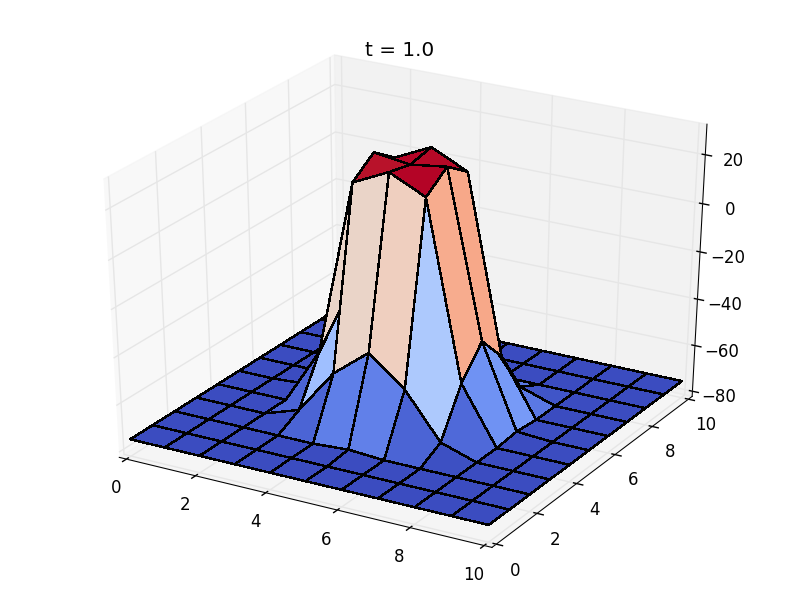
\includegraphics[width=0.9\columnwidth]{examples/example-0401/doc/figures/current_run_l1x1_n10x10_i1_s0_p1__t200.png} 
  \caption{Results, $10 \times 10$ elements, $t=200$}
  \label{example-0401-current-run1-fig}
\end{figure}

\begin{figure}[ht]
  \centering 
  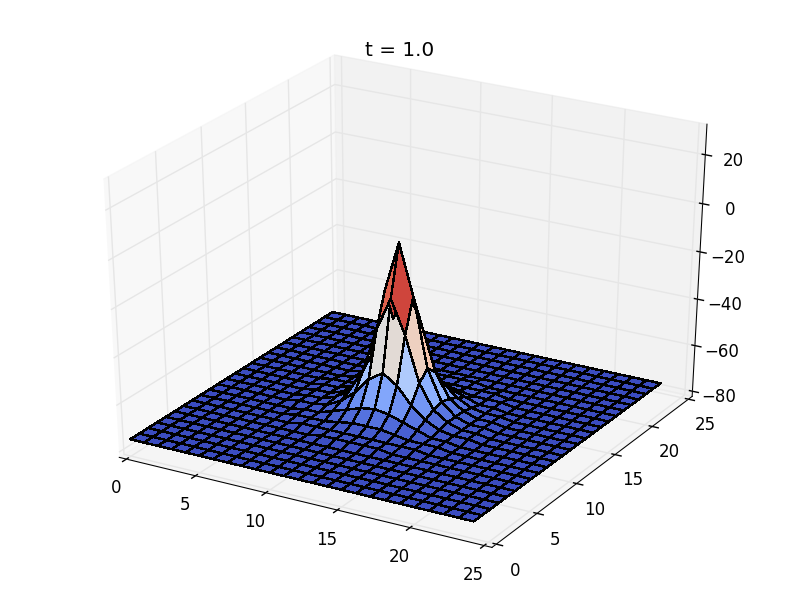
\includegraphics[width=0.9\columnwidth]{examples/example-0401/doc/figures/current_run_l1x1_n24x24_i1_s0_p1__t200.png} 
  \caption{Results, $24 \times 24$ elements, $t=200$}
  \label{example-0401-current-run2-fig}
\end{figure}

\begin{figure}[ht]
  \centering 
  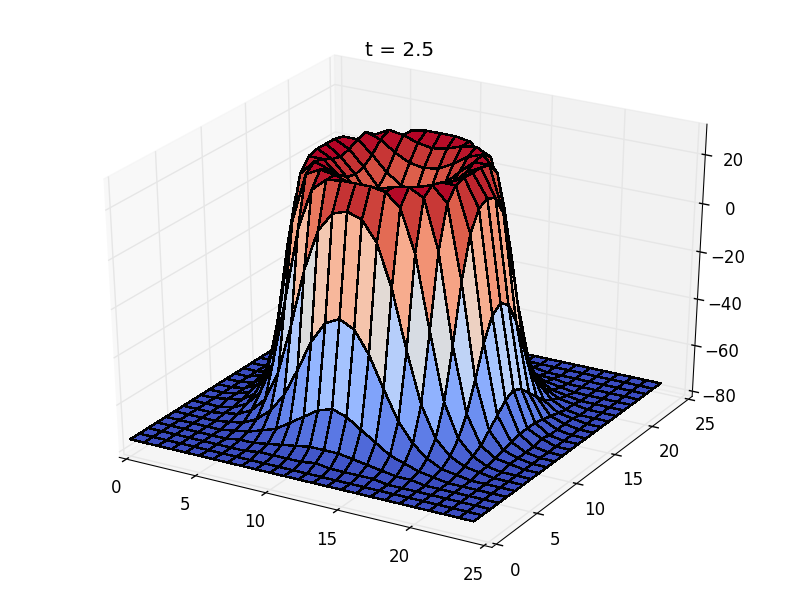
\includegraphics[width=0.9\columnwidth]{examples/example-0401/doc/figures/current_run_l1x1_n24x24_i1_s0_p1__t500.png} 
  \caption{Results, $24 \times 24$ elements, $t=500$}
  \label{example-0401-current-run3-fig}
\end{figure}

%\begin{figure}[h!]
%    \centering 
%    \includegraphics[width=0.9\columnwidth]{examples/example-0001/doc/figures/cheart_reference.eps} 
%    \caption{Results, CHeart reference.}
%    \label{example-0001-cheart-reference-fig}
%\end{figure}
%%
%\begin{figure}[h!]
%    \centering 
%    \includegraphics[width=0.9\columnwidth]{examples/example-0001/doc/figures/iron_reference.eps} 
%    \caption{Results, iron reference.}
%    \label{example-0001-iron-reference-fig}
%\end{figure}
%%
%\begin{figure}[h!]
%    \centering 
%    \includegraphics[width=0.9\columnwidth]{examples/example-0001/doc/figures/current_run_l2x1x1_n8x4x4_i1_s0.eps} 
%    \caption{Results, current run.}
%    \label{example-0001-current-run-fig}
%\end{figure}
%
%===============================================================================
%
\subsubsection{Validation}
%
We compare with a Matlab implementation.
%
%===============================================================================
%===============================================================================
